\documentclass[tikz, border=10pt]{standalone}

% preamble
\usepackage[utf8]{inputenc}
\usepackage[upright]{fourier}
\usepackage{tikz}
\usetikzlibrary{
    matrix,         % tikz's library for drawing matrix
    arrows,         % tikz's library of different arrow styles
    snakes,         % tikz's library of snake arrow: zigzag, coil, ...
    topaths         % tikz's library of various to or edge style
}

% define global unit
\newcommand{\unit}{1 cm}
% define styles
\tikzset{
    special node/.style={circle, minimum size=\unit},
    general node/.style={circle, minimum size=\unit},
    mul arrow/.style={draw, sloped, midway, fill=white},
    plus arrow/.style={midway, sloped, fill=white},
    snake arrow/.style={
        -latex, red, thick,
        snake=zigzag,
        segment length=2.5mm, segment aspect=0,
        segment amplitude=1.5mm, line before snake=1mm,
        line after snake=3mm,
        draw opacity=0.8
    }
}

\begin{document}
    % first picture
    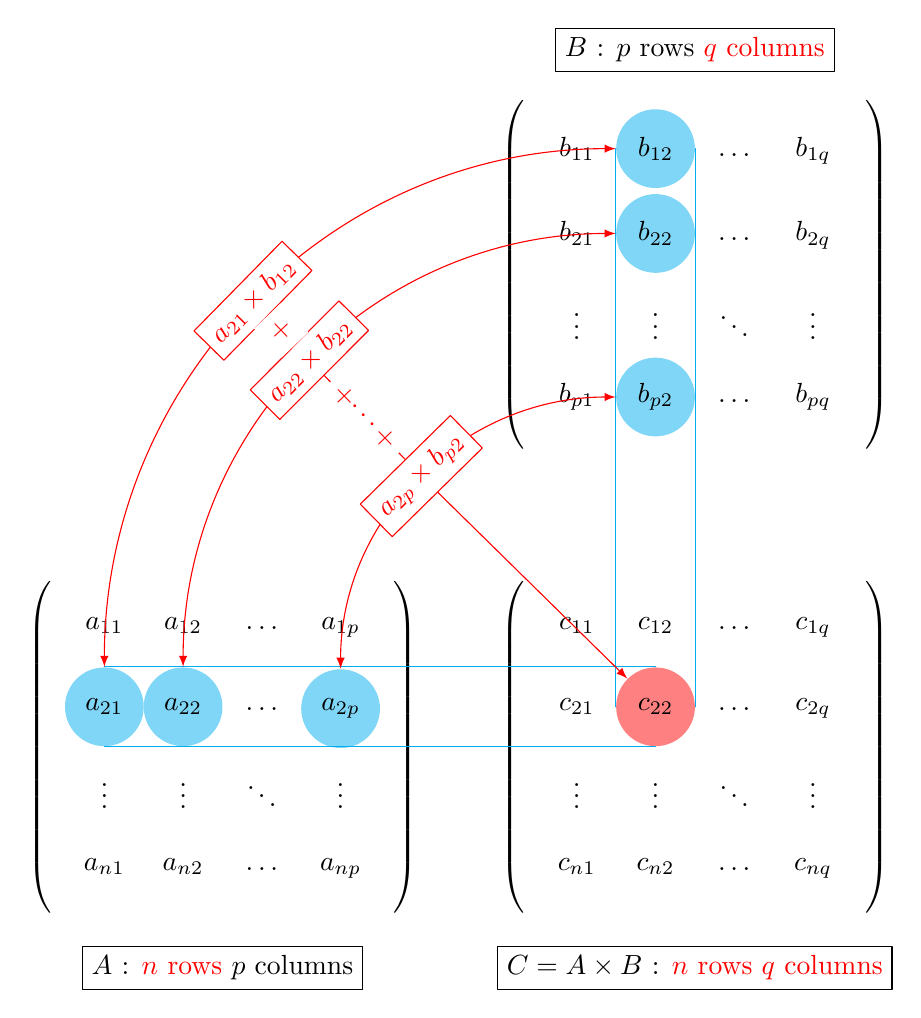
\begin{tikzpicture}[>=latex, cap=round, join=round]
        % matrix A
        \matrix (A) [
            matrix of math nodes,
            nodes = {general node},
            left delimiter  = (,
            right delimiter = )
        ] at (0,0) {
            a_{11} & a_{12} & \ldots & a_{1p}  \\
            |[special node, fill=cyan!50]| a_{21} & |[special node, fill=cyan!50]| a_{22}
            & \ldots & |[special node, fill=cyan!50]| a_{2p} \\
            \vdots & \vdots & \ddots & \vdots  \\
            a_{n1} & a_{n2} & \ldots & a_{np}  \\
        };
        % matrix A's text label
        \node [draw,below=10pt] at (A.south) { $A$ : \textcolor{red}{$n$ rows} $p$ columns};
        
        % matrix B
        \matrix (B) [
            matrix of math nodes,
            nodes = {general node},
            left delimiter  = (,
            right delimiter = )
        ] at (6*\unit,6*\unit) {
            b_{11} & |[special node, fill=cyan!50]| b_{12} & \ldots & b_{1q} \\
            b_{21} & |[special node, fill=cyan!50]| b_{22} & \ldots & b_{2q} \\
            \vdots & \vdots & \ddots & \vdots  \\
            b_{p1} & |[special node, fill=cyan!50]| b_{p2} & \ldots & b_{pq} \\
        };
        % matrix B's text label
        \node [draw,above=10pt] at (B.north) { $B$ : $p$ rows \textcolor{red}{$q$ columns}};

        % matrix C
        \matrix (C) [
            matrix of math nodes,
            nodes = {general node},
            left delimiter  = (,
            right delimiter = )
            ] at (6*\unit,0) {
                c_{11} & c_{12} & \ldots & c_{1q} \\
                c_{21} & |[special node, fill=red!50]| c_{22} & \ldots & c_{2q} \\
                \vdots & \vdots & \ddots & \vdots \\
                c_{n1} & c_{n2} & \ldots & c_{nq} \\
            };
        
        % matrix B's text label    
        \node [draw, below=10pt] at (C.south) {$ C=A\times B$ : \textcolor{red}{$n$ rows} \textcolor{red}{$q$ columns}};
        
        % connecting arrows
        \draw[cyan] (A-2-1.north) -- (C-2-2.north);
        \draw[cyan] (A-2-1.south) -- (C-2-2.south);
        \draw[cyan] (B-1-2.west)  -- (C-2-2.west);
        \draw[cyan] (B-1-2.east)  -- (C-2-2.east);
        \draw[<->, red](A-2-1) to[out=90, in=180] node[mul arrow] (x) {$a_{21}\times b_{12}$} (B-1-2);
        \draw[<->, red](A-2-2) to[out=90, in=180]
        node[mul arrow] (y) {$a_{22}\times b_{22}$} (B-2-2);
        \draw[<->, red](A-2-4) to[out=90, in=180]
	    node[mul arrow] (z) {$a_{2p}\times b_{p2}$} (B-4-2);
        \draw[red, ->] (x) to node[plus arrow] {$+$} (y) to node[plus arrow] {$+\raisebox{.5ex}{\ldots}+$} (z) to (C-2-2.north west);
    \end{tikzpicture}

    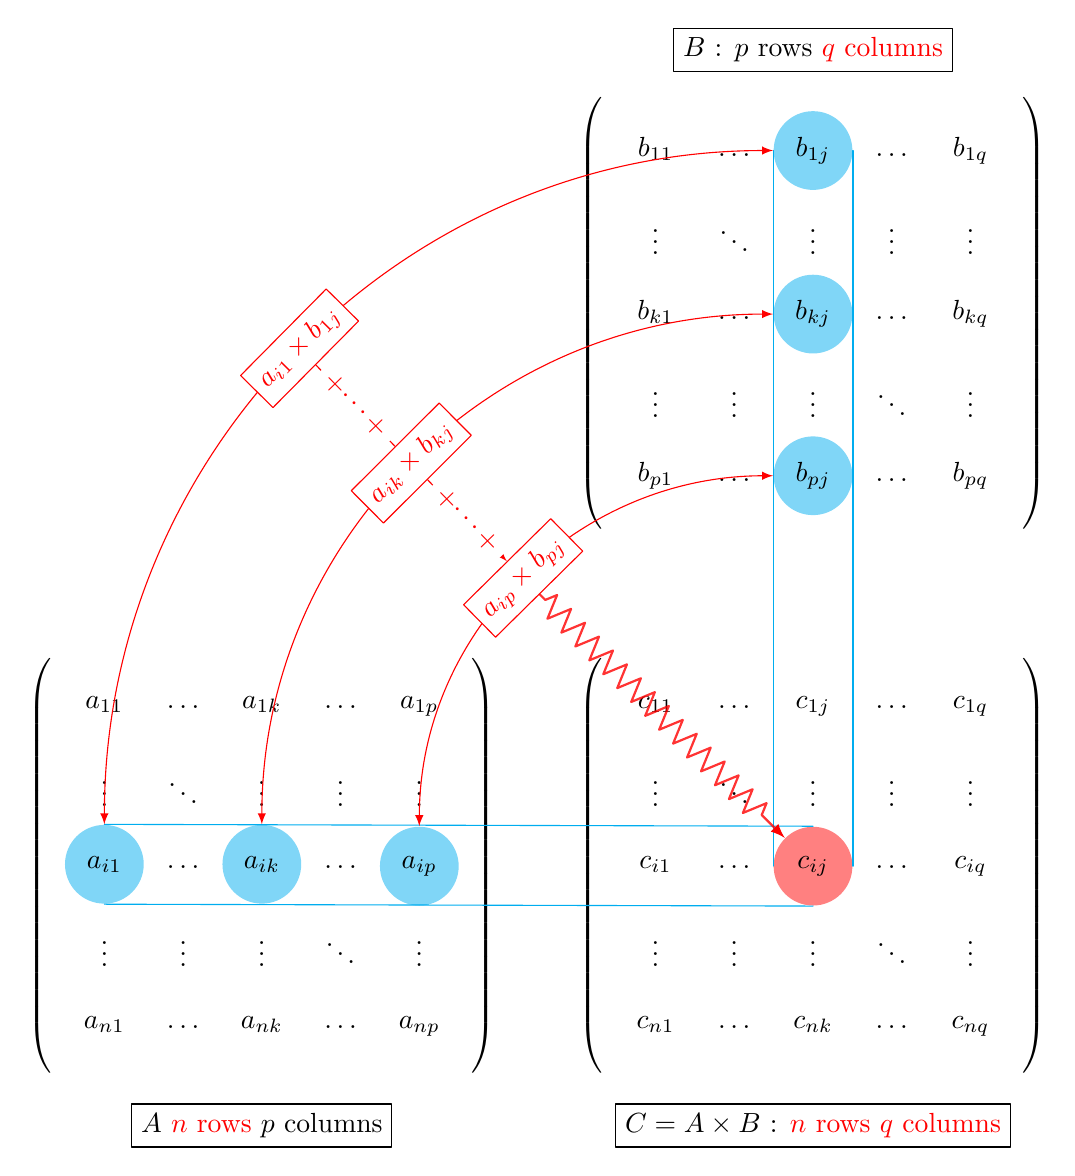
\begin{tikzpicture}[>=latex, cap=round, join=round]
        \matrix (A) [
            matrix of math nodes,
            nodes = {general node},
            left delimiter  = (,
            right delimiter = )
        ] at (0,0) {
            a_{11} &\ldots & a_{1k} & \ldots & a_{1p}  \\
            \vdots & \ddots & \vdots & \vdots & \vdots \\
            |[special node, fill=cyan!50]| a_{i1} & \ldots & |[special node, fill=cyan!50]| a_{ik} & \ldots & |[special node, fill=cyan!50]| a_{ip} \\
            \vdots & \vdots& \vdots & \ddots & \vdots  \\
            a_{n1}& \ldots & a_{nk} & \ldots & a_{np}  \\
        };
        \node [draw, below=10pt] at (A.south) { $A$ \textcolor{red}{$n$ rows} $p$ columns};
        
        \matrix (B) [
            matrix of math nodes,
            nodes = {general node},
            left delimiter  = (,
            right delimiter =)
        ] at (7*\unit,7*\unit) {
            b_{11} &  \ldots& |[special node, fill=cyan!50]| b_{1j} & \ldots & b_{1q}  \\
            \vdots& \ddots & \vdots & \vdots & \vdots \\
            b_{k1} &  \ldots& |[special node, fill=cyan!50]| b_{kj} & \ldots & b_{kq}  \\
            \vdots& \vdots & \vdots & \ddots & \vdots \\
            b_{p1} &  \ldots& |[special node, fill=cyan!50]| b_{pj} & \ldots & b_{pq}  \\
        };
        \node [draw, above=10pt] at (B.north) { $B$ : $p$ rows \textcolor{red}{$q$ columns}};
 
        \matrix (C) [
            matrix of math nodes,
            nodes = {general node},
            left delimiter  = (,
            right delimiter = )
            ] at (7*\unit,0) {
                c_{11} & \ldots& c_{1j} & \ldots & c_{1q} \\
                \vdots& \ddots & \vdots & \vdots & \vdots \\
                c_{i1}& \ldots & |[special node, fill=red!50]| c_{ij}  & \ldots & c_{iq} \\
                \vdots& \vdots & \vdots & \ddots & \vdots \\
                c_{n1}& \ldots & c_{nk} & \ldots & c_{nq} \\
            };
        \node [draw, below=10pt] at (C.south) {$ C=A\times B$ : \textcolor{red}{$n$ rows} \textcolor{red}{$q$ columns}};
 
        \draw[cyan] (A-3-1.north) -- (C-3-3.north);
        \draw[cyan] (A-3-1.south) -- (C-3-3.south);
        \draw[cyan] (B-1-3.west)  -- (C-3-3.west);
        \draw[cyan] (B-1-3.east)  -- (C-3-3.east);
        \draw[<->, red](A-3-1) to[out=90, in=180] node[mul arrow] (x) {$a_{i1}\times b_{1j}$} (B-1-3);
        \draw[<->, red](A-3-3) to[out=90, in=180] node[mul arrow] (y) {$a_{ik}\times b_{kj}$}(B-3-3);
        \draw[<->, red](A-3-5) to[out=90, in=180] node[mul arrow] (z) {$a_{ip}\times b_{pj}$}(B-5-3);
        \draw[->, red] (x) to node[plus arrow] {$+\raisebox{.5ex}{\ldots}+$} (y) to node[plus arrow] {$+\raisebox{.5ex}{\ldots}+$} (z);
        \draw[snake arrow] (z) -- (C-3-3.north west);
    \end{tikzpicture}
\end{document}
